\documentclass[preprint, 12pt]{elsarticle}

% KU requirements
\usepackage[margin=2.5cm]{geometry}
\usepackage{setspace}
\onehalfspacing

% Temporary packages used while editing
\usepackage[usenames,dvipsnames]{color}

% Packages
\usepackage[colorlinks=true]{hyperref}
\usepackage{xspace}
\usepackage[utf8]{inputenc}

% Options
\biboptions{authoryear}

% Custom commands
\newcommand{\Cree}{\emph{Cree}\xspace}

\begin{document}

\begin{frontmatter}

\title{\emph{Cree}: A modern toolbox for readymade economic experiments}
\author{Jonas K. Sekamane}
\journal{Supervised by Ulrik Haagen Nielsen.}
\address{{\color{red} First draft}}

\begin{abstract}
{\color{red} ...}
\end{abstract}
%\begin{keyword}Science \sep Publication \sep Complicated\end{keyword}

\end{frontmatter}


%% main text
\section{Introduction}
\label{S:Introduction}

This paper introduces a modern toolbox for readymade economic experiments called \Cree. \Cree takes advantage of the great advances in technology, in particular the new types of devices (smart-phones, tablets) and the availability of general-purpose software libraries. 

The great merit of \Cree is the very few restrictions it places on the equipment facing subjects. Few restrictions clear the way for much broader participation, strengthening the external validity of any experiment. \Cree experiments can be run in a myriad of settings, including laboratories, but also in \emph{extra-laboratory} settings such as classrooms, workplaces, or over the Internet \citep{Charness_Gneezy_Kuhn_2013}. With \Cree the computer-equipped laboratory is no longer a necessity -- lowering the overall costs of conducting economic experiments. The researcher can still choose to provide subjects with devices, but can just as easily let subjects use their own devices. 

\Cree is build using web technologies. Content is structured using the markup language \emph{HTML}. The layout and presentation across different screen sizes is archived with the style sheet language \emph{CSS}. And all logic is constructed using the programming language \emph{JavaScript}. All web browsers interpret these three cornerstone languages and render pages accordingly. Subjects participate in \Cree experiments though a web browser. Because \Cree is fundamentally native to the web browser, it avoids many of the restrictions, that other toolboxes suffer from.

In addition there is a vibrant ecosystem surrounding these web technologies. \Cree exploits this ecosystem and takes full advantage of the software libraries that exist. This provides stability, flexibility, and makes it easy to set up and run economic experiments. Fore instances, \Cree uses the software library \emph{Node.js} to run the server and handle networking issues. The asynchronous architecture of \emph{Node.js} gives \Cree the flexibility to handle real-time events, which many other toolboxes is not capable of. With this flexibility \Cree can run everything, from simple dictator game experiments, to highly sophisticated auction experiments. \Cree is a framework that provides the tools to handle many of the otherwise mundane, complicated or manually tasks required to set up and run economic experiments.

Technological advances opens up a new path, however the path is not without obstacles. This paper explores and discusses how to handle these obstacles. Some obstacles are alleviated through appropriate technical design of the toolbox. Other obstacles require actions taken by the researcher.

{\color{red}... Explain why you repeatedly refer to studies on Mechanical Turk ...}

\section{Requirements}
\label{S:Requirements}

\subsection{System requirements}
% What are the system requirements for \Cree?

\Cree requires a server, ie. any computer with \emph{Node.js} installed\footnotemark[1]. \Cree has several dependencies -- because it is built on general-purpose software libraries -- however all of these dependencies are automatically installed, or come pre-bundled, with \Cree. The server will need to be connected to the devices used by the subject, either through the internet or though a local network (eg. WiFi). 

\begin{figure}[h!]
  \caption{Schematic overview of the network setup with server and clients}
  \centering
    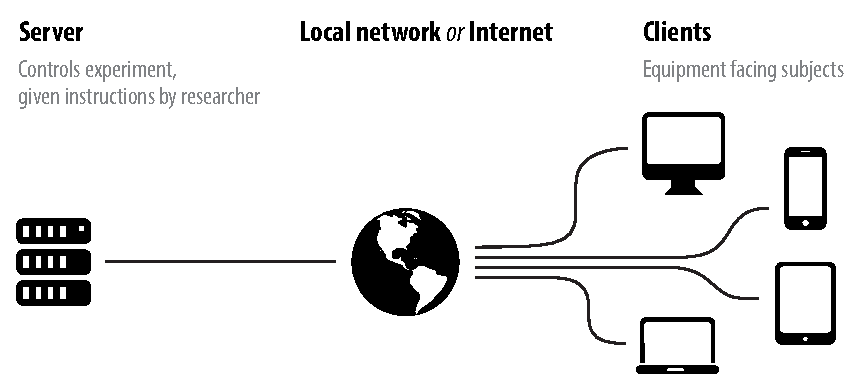
\includegraphics[width=\textwidth]{figures/setup}
\end{figure}

Subjects access \Cree experiments though an web browser. Any modern web browser will suffice\footnotemark[2], which means that subjects can participate in experiments using smart-phones, tablets, or any computer (Windows, Mac, Linux). Every subject will need a device. The researcher can choose to provide devices, or have subjects use their own personal devices.

\footnotetext[1]{Node.js is easily installed from \url{http://nodejs.org}.}

\footnotetext[2]{A modern web browser is either: IE version 9+, Chrome current version, Firefox current version, OSX Safari version 5.1+, Opera version 12.1+, iOS Safari version 6.1+, or Android Browser version 4.0+. The browser must allow JavaScript, which all browsers due by default. \Cree automatically check that these requirements are met, before the subject is allowed to enter the experiment.}

\subsection{Alternative toolboxes}
% What are the alternative toolboxes and how do they compare to Cree?

\emph{z-Tree} is currently the commonly used toolbox for conducting economic experiments. The development of \emph{z-Tree} started in 1995 and has been updated continuously \citep{Fischbacher_2007}. However the foundation and guiding principles of \emph{z-Tree} is based on the technology that was available two decades ago. Several other toolboxes exist that can run economic experiments. Below I divide the the toolboxes into four categories based on the restrictions they places on the equipment facing subjects:

\begin{table}[h!]
\begin{tabular}{ l p{0.7\textwidth} }
{\bf Application:} & z-Tree, E-Prime, ESI/ICES Software \\
{\bf Requires Python:} & UAA-PEET \\
{\bf Requires Java:} & BoXS, EconPort, Multistage, Comlab, Aton, JessX, JAuctions, JMarkets, SWIEE \\
{\bf Browser native:} & SoPHIE, Willow, jsPsych, Tatool, QRTEngine, WebExp, WEXTOR, VeconLab \\
\end{tabular}
\end{table}

Toolboxes, such as \emph{z-Tree}, are applications. They are written for a specific operating system, and will only run on that specific operating system. All toolboxes in this category requires Microsoft Windows. These applications are not easily ported to other computer operating systems. And they will require a complete restructuring -- focused on optimising screen sizes and battery life -- if they are every to run on smart-phones or tablets. In addition, applications will have to be downloaded (and installed) on the computer facing subjects, before they can participate in experiments. This requirement hinders subjects from using their personal devices.

The second category contains toolboxes written in \emph{Python}. Python is platform independent, so these toolboxes can run on several operating systems, but they require that Python is installed on the equipment facing subjects\footnotemark[3]. These toolboxes also require downloading software.

\footnotetext[3]{Python can be packaged into stand-alone applications. These stand-alone applications can run on equipment where Python is not installed.}

Toolboxes in the third category are written in \emph{Java}. These are less restrictive, since subjects can participate in experiments though a web browser that has the Java-plugin. Thus there is no need to predownload or preinstall software on the equipment facing subjects. While the Java-plugin is widely distributed, it is not universal\footnotemark[4]. And increasing concerns regarding security issues with the Java-plugin has lead browsers manufactures to implement various warnings and hindrances\footnotemark[5]. 

\footnotetext[4]{A Millward Brown survey from 2011 found a penetration rate of 73\% on PCs in mature markets. Source: \url{http://www.adobe.com/mena_en/products/flashplatformruntimes/statistics.html}. This is also mimicked on the server-side with only 0.1\% of websites using Java. Source: \url{http://w3techs.com/technologies/overview/client_side_language/all}. The Java-plugin is not supported on iOS nor Android. Source: \url{http://www.java.com/en/download/faq/java_mobile.xml}.}
 
\footnotetext[5]{Eg. due to security concerns by default the Java-plugin is disabled in Google Chrome version 42 (released April 2015). Source: \url{https://www.java.com/en/download/faq/chrome.xml}.}

The fourth category of toolboxes run natively in the web browser, without the need for any browser plug-ins or predownloaded software. These toolboxes place the same low restrictions on the equipment facing subjects as \Cree. However, none of these toolboxes currently support simultaneous real-time interaction between subjects -- ie. it is impossible to design experiments where subjects continuously provide input, while continuously and simultaneously receives feedback from the other subjects. Some toolboxes support sequential decision making, while others completely lack interaction among subjects.


\section{Running experiments}
\label{S:Running}

\subsection{Recruitment}
% How are subjects recruited?

The method used to recruit subjects will depend on the type of experiment and the desired representativeness of subjects. 

It is commonly assumed that subjects are \emph{naïve}, eg. encounter the experimental material for the first time, and have no a priori knowledge of the experiment, the purpose, nor knowledge of related experiments. This is not true for experiments conducted over the internet, and is often misapprehended by researchers, as shown by \citet*{Chandler_Mueller_Paolacci_2014}. They investigate experiments where subjects are recruited through Amazon's \emph{Mechanical Turk} system. \emph{Mechanical Turk} is a crowdsourcing platform of 500,000 workers that perform mostly small tasks and are paid a piece rate. Every worker has an account, and \emph{Mechanical Turk} prevents an account from preforming the same task twice. \cite{Chandler_Mueller_Paolacci_2014} find that: 

\begin{enumerate}
\item subjects have experience from related experiments. By pooling 16,408 observations (or completed tasks) across 132 studies, they find just 7,498 unique subjects -- averaging 2.24 observation per subject. The 10\% most prolific subjects account for 41\% of all observations. In addition \cite{Chandler_Mueller_Paolacci_2014} survey 300 workers on \emph{Mechanical Turk} and find that 56\% have previously been exposed to the \emph{Prisoner's dilemma} and 52\% to the \emph{Ultimatum game}. 
\item subjects share information about experiments. About one fourth of workers in the \cite{Chandler_Mueller_Paolacci_2014} survey respectively report they know other workers in person, and that they read or discuss \emph{Mechanical Turk} online on blogs and forums. The focus of the conversation is typically not the specific contents of the experiment, but rather pay rates and reputation. \cite{Chandler_Mueller_Paolacci_2014} conclude that researchers should be particular aware of cross talk, when information can increase financial rewards -- such as when using techniques to increase attention (\emph{instructional manipulation checks}, or \emph{got-cha} questions), or when using techniques to deny payment. They suggest that researchers asks subjects how they found the experiment, and monitor discussion boards that refer a lot of subjects to the experiment.
\item few subjects attempt to participate repeatedly in the same experiment. Amazon forbids multiply or \emph{sock-puppet} accounts, and actively enforces this policy. \cite{Chandler_Mueller_Paolacci_2014} find 1.2\% of subjects share IP adresses as well as demographic characteristics -- eg. possible \emph{sock-puppet} accounts. They attribute the low percentage to the active enforcement by Amazon.
\end{enumerate}

Internet experiments in general and \emph{extra-laboratory} experiments, are likely to face similar issues. Especially considering \citet*{Goodman_Cryder_Cheema_2013} find that, in all the studies they looked at, \emph{Mechanical Turk} subjects are not significantly different from traditional samples, except one study (on risk aversion).

\Cree does not include a prescreening system to manage the pool of subjects, so recruitment is handled manually by the researcher. The selection process is crucial, and researchers should carefully consider the degree to which subjects can self-select into experiments, since this may invalidate the underlying assumption of naïve subjects. \Cree automatically logs referrals from other websites. And researchers can restrict \Cree so it only accepts one subject per IP address, creating additional protection against subjects participating multiple times in the same experimental session.

\subsection{Coordinated joining}
% How do subjects join an experiment and how to coordinate subjects?

When the researcher initiates the experiment, \Cree returns the URL adresses, that subjects use to join the experiment. Two URLs are displayed, since subjects can participate over the internet and through the local network. URLs should be distributed accordingly. The researcher distributes the URL to participants (via printed hand-outs, e-mail, third-party recruitment system, etc). Subjects join the experiment simply by clicking a link, or by typing the URL into their web browser. \Cree automatically tests if the server can connect to the internet, if this fails then \Cree only displays the local network URL\footnotemark[6]. 

\footnotetext[6]{\Cree does not test whether access to the server is blocked by a firewall, nor if the two required ports are open.}

Besides recruitment and distribution of adresses, there is coordination. In experiments where subjects interact with each other in real-time, the researcher must coordinate subjects so they start the experiment simultaneously. The researcher can specify that \Cree should wait for sufficiently many subjects to join, before starting the session. Ie. the first subject joining will be put on hold, until the last required subject joins. Subjects have limited patience, so the researcher needs to coordinate subjects on a very narrow interval of only a few minutes. There are a couple of different approaches that the researcher can take here. In laboratory experiments it is common to invite more participants than needed for a given session (due to ``no shows''). This option is also possible in \Cree, since \Cree turns down subjects once a session is filled. There is a semi-continues option that expands the interval. Fore instance in the \emph{Prisoner's dilemma} it is common with only two subjects interacting with each other. So instead of waiting for all subjects to join the session, the semi-continuous option will start whenever two new subjects join. However with this option the researcher losses the ability to randomise subjects, ie. pair a subject with another. The lack of randomisation may lead to reciprocity among subjects. There is a third fully-continuous option, where the server simply restarts the experiment after each session. This option can be used in conjunction with fewer subjects per session. If subjects show up late for the first session, they wait for the session to end, whereafter they can join the second session, and so on. All of this continues until the researcher manually stops the experiment.

\subsection{Stability}
% Is Cree stable?

A main priority for researchers is that the software they use to run experiments is stable. Crashes are not only costly and time consuming, but also detrimental to the researcher's reputation among the participating subjects. 

There are two stability objectives; The first is eliminating software bugs, ie. faults causing the software to preform in an unintended or unanticipated manner, and due to the error of the programmer. The second is sufficient error handling, ie. implementing fallbacks to deal with mishaps, so crashes are mitigated, or at the very least an emergency landing is preformed.

Both stability aspects require thorough testing and running countless experiments using the software. \Cree does not have a 20-year track record like \emph{z-Tree}, but nor is it build from scratch. The software libraries and dependencies on which \Cree is build, have been tested intensively by their respective communities. Some libraries are used daily across millions of websites\footnotemark[7]. This speaks volumes to the infrequency of software bugs in the foundation of \Cree.

\footnotetext[7]{The JavaScript library \emph{jQuery} is used on 64.4\% of monitored websites. There is no statistics on the \emph{Bootstrap} CSS library, but its complementary JavaScript library is used on 7.7\% of websites. Source: \url{http://w3techs.com/technologies/overview/javascript_library/all}. While \emph{Node.js} is used as web-server on 0.1\% of monitored websites. Source: \url{http://w3techs.com/technologies/overview/web_server/all}.}

With numerous interconnected and simultaneously used devices, eventually a device will malfunction or the network will suffer a temporary disturbance. \Cree handles these types of errors by allowing subjects that briefly disconnects, to reconnect and continue the experiment. Disconnects and reconnects are logged, so the researcher can later determine if it significantly impacted the results in the current stage of the experiment. \Cree does not reconnect subjects after lengthy disconnects, since this would hold up the entire experiment and adversely impact the waiting time of the other participating subjects. In these instances the experiment proceeds without the disconnected subject.

If subjects attempt to abort the experiment untimely, \Cree displays a warning message. The occurrence of these warning messages are logged. In addition \Cree logs when the subject's web browsers is out of focus\footnotemark[8] -- this is a proxy measure for inattention. The figure below plots the session of one subject. The figure includes connection, disconnection, the stages of the experiment, and periods of inattention (areas shaded red). The full lines mark the beginning of a new stage. The dotted lines are where the subject waits for the other participant.

\begin{figure}[h!]
  \caption{Example of a session timeline of a subject}
  \centering
    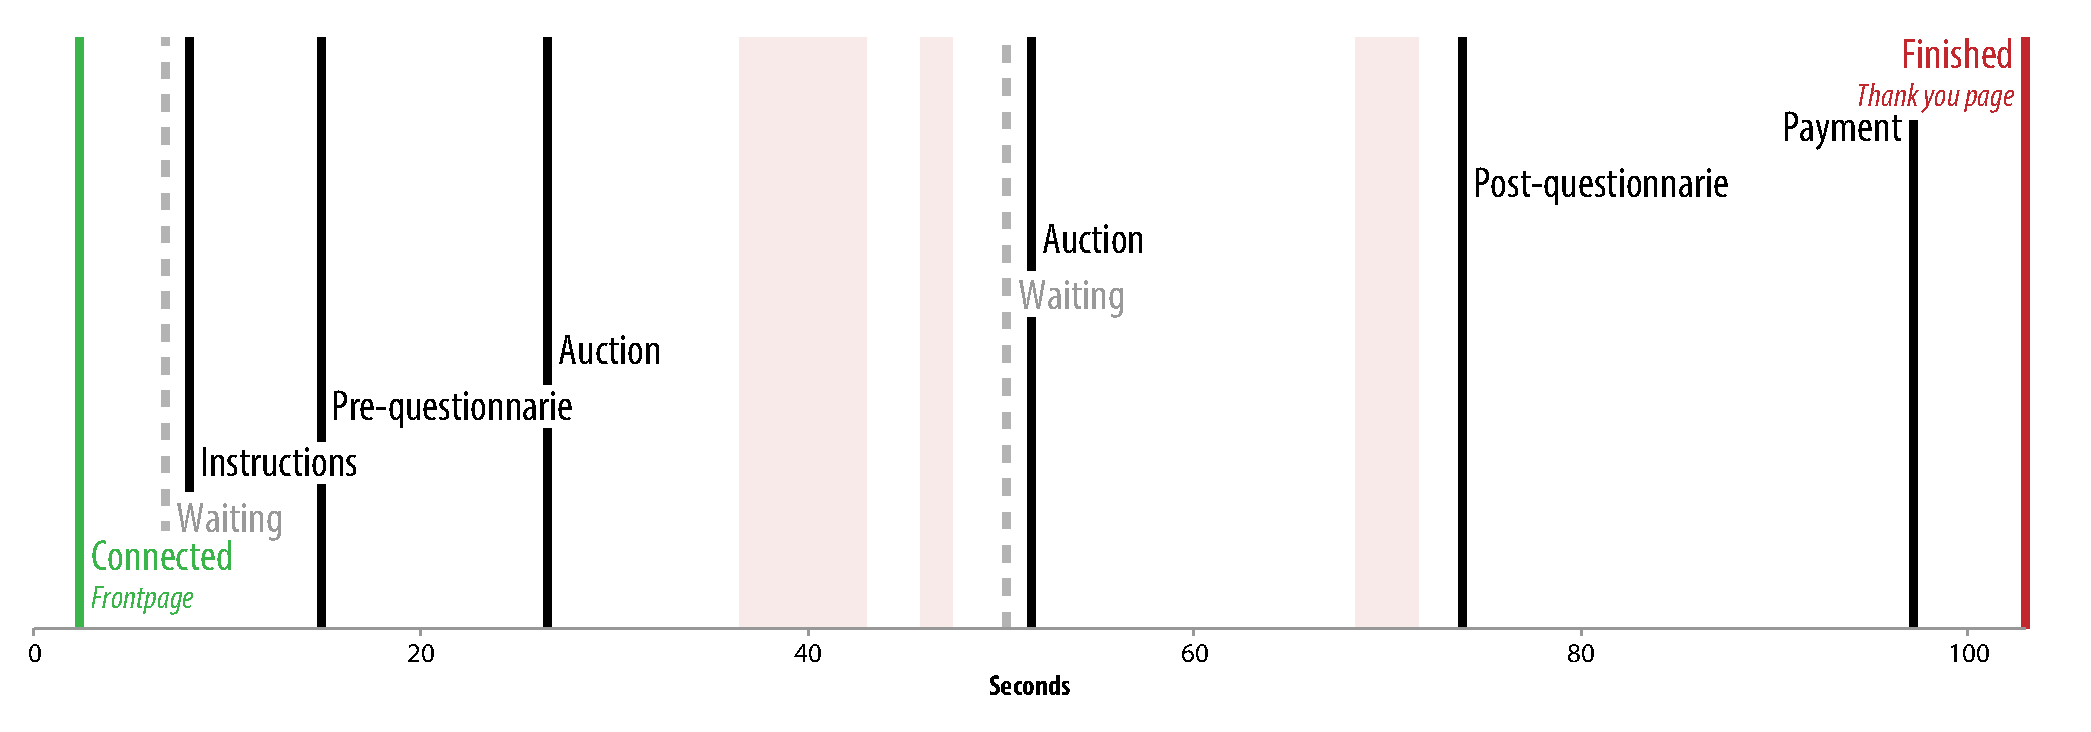
\includegraphics[width=\textwidth]{figures/example_session}
\end{figure}

\footnotetext[8]{ie. when the subject is using a different tab in the web browser, when the web browser is minimised or fully obscured by another application, or when the device enters its power saving or screensaver mode (lock screen on smartphones). Source: \url{http://www.w3.org/TR/page-visibility/}}

\subsection{Duration and supervision}
% Can you run hour-long experiments over the internet (eg. after how long to unsupervised subjects stop paying attention)?

Laboratory experiment can often last an hour or more. There is very little literature on how unsupervised subjects preform in  experiments with long sessions. 

Using \emph{instructional manipulation checks} \citet*{Oppenheimer_Meyvis_Davidenko_2009} show that student subjects pay less attention when unsupervised.

\cite{Goodman_Cryder_Cheema_2013} argue that \emph{Mechanical Turk} may not be appropriate for long or complicated experiments. They compare the results of their experiment -- which lasted about 16 minuts -- to that of \citet*{Paolacci_Chandler_Ipeirotis_2010} that only lasted around 5 minutes. Unlike \cite{Paolacci_Chandler_Ipeirotis_2010} they find that subjects from \emph{Mechanical Turk} are less attentive. They test attentiveness using \emph{instructional manipulation checks} at the end of the survey.

\citet*{Farrell_Grenier_Leiby_2014} run an hour-long experiment on \emph{Mechanical Turk} where subjects fulfil orders (sandwich orders or unspecified product orders). They find that \emph{Mechanical Turk} subjects exert the same amount of effort (or more), and make the same amount of mistakes (or fewer), than student participants. Even in the treatment where \emph{Mechanical Turk} subjects are paid one-fifth of the student participants, where tasks are less intrinsically interesting, and where their wage rate is independent of performance (flat rate of \$5).

The results of \cite{Farrell_Grenier_Leiby_2014} may be due to the selection process, ie. the \emph{Mechanical Turk} subjects that volunteer for their experiment, are more motivated by financial incentives, than other individuals. An indication of this is that 73\% report `extra income' and 28\% report `enterainment' as reasons for using \emph{Mechanical Turk}. Whereas in the \cite{Paolacci_Chandler_Ipeirotis_2010} study it is respectively 61\% and 41\%. Similarly in a short survey by \cite{Williamson_2014} on \emph{Mechanical Turk} only 28.9\% respond that they would be willing to participate in a hour-long follow-up interview for an additional \$15.

In sum the researcher needs to carefully consider the selection process, to ensure that subjects are representative and that results have general validity. When subjects ability to self-select into experiments is restricted, it remains unclear if subjects will participate in hour-long experiments, and it is unclear how attentive they are during these long unsupervised sessions.

There are two alternative approaches, regarding time and duration, that the researchers might consider when designing the experiment. One is the approach of \citet*{Pettit_Friedman_Kephart_Oprea_2014} which speeds up the adjustment process by allowing subjects to continuously change and adapt strategies. They refer to one study where distinctive, long-term implications are observable in rounds lasting only 120 seconds. The other approach, suggested by \cite{Charness_Gneezy_Kuhn_2013}, is to create long time-series data, ie. by recalling subjects every day, week or month. In a traditional laboratory experiment, this would be time consuming and highly inconvenient for subjects, but less so in extra-laboratory settings such as classrooms or over the internet. \cite[p. 96]{Charness_Gneezy_Kuhn_2013} argue that \emph{``the classic 10–20 period repetition of the public-goods game may not be a good analog for the expression of preference for tax policy that citizens make when they vote every couple of years''}. \Cree can execute both alternative approaches, since it allows real-time interaction among subjects and works in \emph{extra-laboratory} settings.


\section{Expected results}
\label{S:Results}

\section{Designing experiments}
\label{S:Designing}

\section{Conclusion}
\label{S:Conclusion}


%% References
\bibliographystyle{apalike}
\raggedright
\singlespacing
\bibliography{references.bib}

\end{document}